\section{DCR}

% \begin{frame}
%     \frametitle{Overview of Duration Consistency Alignment}
%     The Duration Consistency Alignment module aims to enhance the temporal consistency of the dubbed audio.
%     \begin{itemize}
%         \item \textbf{Method:} Achieve optimal alignment of phoneme-level durations through lip motion feature extraction and dynamic programming algorithms. It is mainly divided into three parts:
%     \end{itemize}
%     \begin{columns}[T] % Use top-aligned two columns
%         \column{0.55\textwidth} % Left column width is 55% of the text width
%         \textbf{Module Composition:}
%         \begin{itemize}
%             \item \textbf{Lip Motion-Phoneme Alignment:} Extract lip motion features and compute the similarity matrix with phoneme features.
%             \item \textbf{Phoneme Duration Expansion:} Use dynamic programming to find the optimal alignment and expand phoneme durations.
%             \item \textbf{Mel-Spectrogram Duration Expansion:} Expand the length of the mel-spectrogram based on audio duration.
%         \end{itemize}
%         \column{0.3\textwidth} % Right column width is 45% of the text width
%         \begin{figure}[htpb]
%             \centering
%             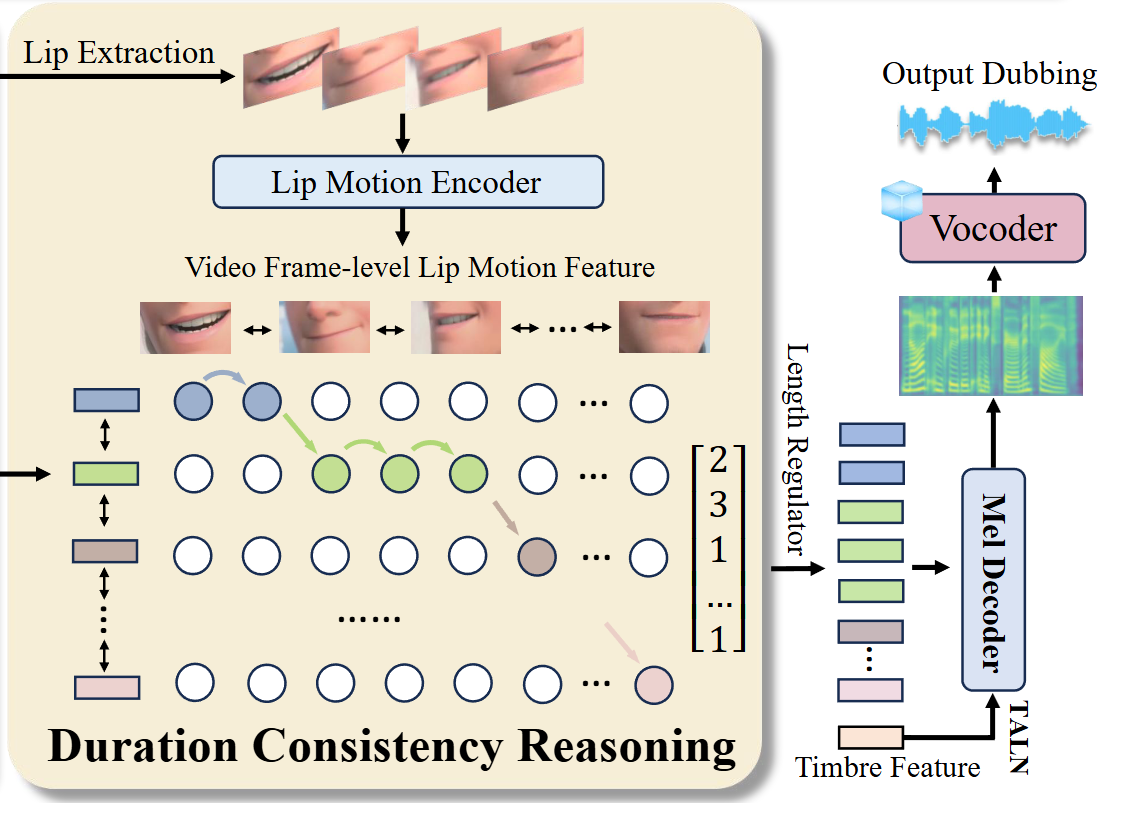
\includegraphics[width=\linewidth]{figs/DCR.png} % Replace with your image path
%             \caption{Illustration of the DCR module}
%             \label{fig:dcr-diagram}
%         \end{figure}
%     \end{columns}
% \end{frame}
\begin{frame}
    \frametitle{Overview of Duration Consistency Alignment}
    \textbf{Objective:} Enhance temporal consistency of dubbed audio.
    \begin{columns}[T] % Use top-aligned two columns
        \column{0.55\textwidth} % Left column width is 55% of the text width
        \textbf{Module Composition:}
        \begin{itemize}
            \item \textbf{Lip Motion-Phoneme Alignment:} Extract lip motion features and align with phoneme features.
            \item \textbf{Phoneme Duration Expansion:} Use dynamic programming to optimize phoneme durations.
            \item \textbf{Mel-Spectrogram Duration Expansion:} Adjust mel-spectrogram length based on audio duration.
        \end{itemize}
        \column{0.3\textwidth} % Right column width is 30% of the text width
        \begin{figure}
            \centering
            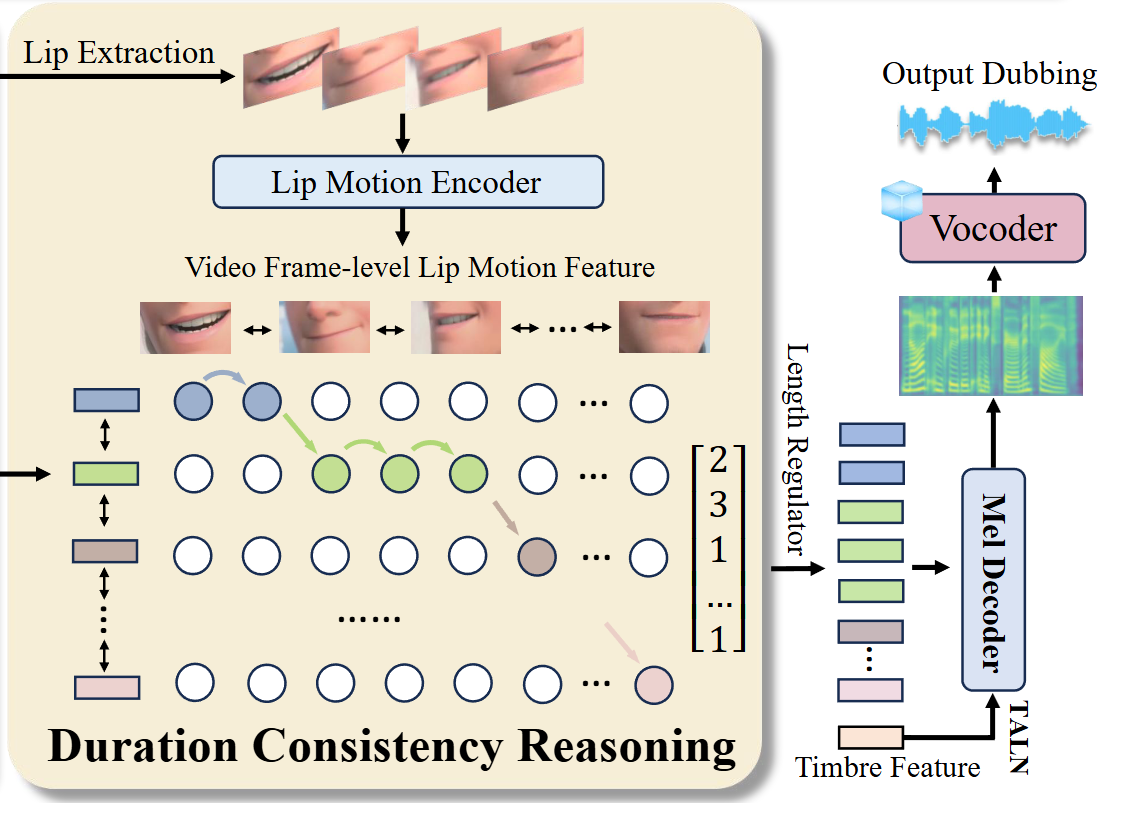
\includegraphics[width=\linewidth]{figs/DCR.png} % Replace with your image path
            \caption{DCR module illustration}
            \label{fig:dcr-diagram}
        \end{figure}
    \end{columns}
\end{frame}


\begin{frame}{Duration Consistency Alignment (DCR)}
\framesubtitle{(1) Lip Motion-Phoneme Alignment}
\begin{itemize}
    \item \textbf{Step 1: Lip Motion-Phoneme Alignment}
    \begin{itemize}
    \item \textbf{Objective:} Extract lip motion features from the reference video and align them with phoneme features.
    \item \textbf{Steps:}
    \begin{enumerate}
        \item Extract the lip motion region from the video:
        \begin{equation}
            V_{\text{lip}} \in \mathbb{R}^{L_v \times H_{\text{lip}} \times W_{\text{lip}} \times C}
        \end{equation}
        \item Obtain the lip motion representation using a lip motion encoder:
        \begin{equation}
            E_{\text{lip}} \in \mathbb{R}^{L_v \times d_{\text{model}}}
        \end{equation}
    \end{enumerate}
\end{itemize}
\end{itemize}

\end{frame}

\begin{frame}{Duration Consistency Alignment (DCR)}
\framesubtitle{(2) Phoneme Duration Expansion}
\begin{itemize}
    \item \textbf{Step 2: Phoneme Duration Expansion}
    \begin{itemize}
    \item \textbf{Objective:} Expand phoneme durations to match lip motion features.
    \item \textbf{Steps:}
    \begin{enumerate}
        \item \textbf{Similarity Matrix Calculation:} Compute the similarity matrix between phoneme-level acoustic features and lip motion features.
        \begin{equation}
            S_{\text{pho,lip}} = \text{Similarity}(T_a^i, E_{\text{lip}}^j)
        \end{equation}
        \item \textbf{Dynamic Programming Alignment:} Use dynamic programming to find the optimal alignment.
        \begin{equation}
            A_{i,j} = 
            \begin{cases} 
                \text{None}, & \text{if } i > j \text{ or } j - i < L_p - L_{\text{p}} \\
                \max(A_{i-1,j}, A_{i-1,j-1}) + s_{i,j}, & \text{otherwise}
            \end{cases}
        \end{equation}
    \end{enumerate}
\end{itemize}
\end{itemize}
\end{frame}


\begin{frame}{Duration Consistency Alignment (DCR)}
\framesubtitle{(3) Mel-Spectrogram Duration Expansion}
\begin{itemize}
    \item \textbf{Step 3: Mel-Spectrogram Duration Expansion}
    \begin{itemize}
    \item \textbf{Objective:} Expand the length of the mel-spectrogram to match the audio duration.
    \item \textbf{Steps:}
    \begin{enumerate}
        \item \textbf{Fixed Ratio Relationship:} Expand the length of the mel-spectrogram based on audio duration.
        \begin{equation}
            n = \frac{L_{\text{mel}}}{L_0} = \frac{sr/hs}{FPS} \in \mathbb{N}^*
        \end{equation}
        \item \textbf{Mel-Spectrogram Generation:} Use a length regulator to generate the mel-spectrogram of the desired length:
        \begin{equation}
            \tilde{A}_{\text{Dub}} = \text{Vocoder}(\text{MelDecoder}(LR(T_a, A^* \times n), E_{\text{imbr}}))
        \end{equation}
    \end{enumerate}
\end{itemize}
\end{itemize}
\end{frame}